\section{Shape}
\subsection{Type definitions}
The following type definitions are made:
\begin{codelisting1}
	typedef int                 _int_t;
	typedef int                 _coord_t;
	typedef std::vector< int >  _halo_t;
	typedef std::array<int, 3>  _vector_t;
\end{codelisting1}
\subsection{Halos}
\label{section_shape_halos}
\begin{figure}%{o}{0.6\textwidth}
	\centering
	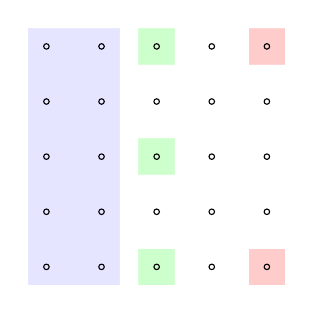
\begin{tikzpicture}[scale=0.7]
	\def\max{5}
	\def\margin{0.33}
	\draw [white, fill=blue,  opacity=0.1] (1-\margin,1-\margin) rectangle (2+\margin,\max+\margin);
	\foreach \y in {1,3,...,\max}
	\draw [white, fill=green, opacity=0.2] (3-\margin,\y-\margin) rectangle (3+\margin,\y+\margin);
	\foreach \y in {1,5,...,\max}
	\draw [white, fill=red, opacity=0.2] (5-\margin,\y-\margin) rectangle (5+\margin,\y+\margin);
	\foreach \x in {1,...,\max}
	\foreach \y in {1,...,\max}
	\draw (\x,\y) circle (0.05);
	\end{tikzpicture}
	\label{figure_halo_structure_41}
	\caption{\footnotesize{Halo structure for \texttt{\_halo\_t halo\_property = \{2, 1, 1\}}: two lines of coarseness 0 (entirely occupied), one line of coarsenesses 1 and 2, respectively. The resulting halo size is \texttt{halo\_size = 5.}}}
\end{figure}
The form of the halos is referred to as \verb|halo_property| and can be defined using the aforesaid typedef. The \verb|int| at position 0 hereby indicates the number of lines to be sent entirely, the \verb|int| at index 1 represents the number of lines coarsened by the factor $2^1$ et cetera. Thus at index $i$ is given the number of lines for the coarseness $2^i$. In the following we identify $i$ as the order of coarseness. See figure \ref{figure_halo_structure_41} for an example. The term \verb|halo_size| indicates the overall number of halo layers and is calculated iteratively as
\begin{align}
	\label{eq_halo_size_41}
	\text{\footnotesize\texttt{halo\_size}}_0 =& \quad \text{\footnotesize\texttt{halo\_property[0]}} \\
	\text{\footnotesize\texttt{halo\_size}}_n =& \left( \frac{ \text{\footnotesize\texttt{halo\_size}}_{n-1} +1}{2^n} + \text{\footnotesize\texttt{halo\_property[n]}} \right) \cdot 2^n + 1. \nonumber
\end{align}

\subsection{Domain dimensions}
\label{section_shape_dom_dims}
We name disaggregated all the classes that are split up among the MPI processes, like \verb|Process_domain| and \verb|Operator|. In this context, \verb|global_size| denotes the size of the objects' overall conjunction. We define \verb|begin| of a dissaggregated object as the tuple containing the object's smallest index in each dimension and \verb|end| the tuple of smallest indeces outside the object. With this it is possible to calculate an object's \verb|domain_size| as the difference between its end and begin in each dimension. Eventually each object has its \verb|total_size| which adds the surrounding halo layers in each dimension. Consequently it consists of the \verb|domain_size| + 2 * \verb|halo_size| in each dimension.

\begin{figure}[h]
	\def\sca{0.8}
	\begin{tikzpicture}[scale=\sca, , every node/.style={scale=\sca}]
	\def\halosize{1}
	\def\xo{1}
	\def\yo{1}
	\def\xi{7}
	\def\yi{7}
	\def\otherxo{2}
	\coordsys[0][0][$x_\text{global}$][$y_\text{global}$][16][8.5] \par
	\xtick[\xo+\halosize][-0.1][0.1][$x_0$] \par
	\ytick[\yo+\halosize][-0.1][0.1] \par
	\xtick[\xi][-0.1][0.1][$x_1$] \par
	\ytick[\yi][-0.1][0.1][$y_1$] \par
	\coordsys[\halosize+0.5][\halosize+0.5][$x_\text{domain}$][$y_\text{domain}$][\xi+1.6][8.5] \par
	\xtick[\xo+\halosize][\halosize+0.4][\halosize+0.6][$ $] \par
	\node [below right]at (\xo+\halosize-0.15, \halosize+0.55) {0};
	\ytick[\halosize+1][\halosize+0.4][\halosize+0.6][$ $] \par
	\node [above left] at (\xo+0.6, \halosize+0.95) {0};
	\draw [fill=green, opacity=0.05] (\xo-0.5, \yo-0.5) rectangle (\xi+0.5, \yi+0.5);
	\draw [decorate,decoration={brace,mirror,amplitude=10pt},xshift=0pt,yshift=0pt]
	(\xi+0.5,\yo-\halosize+0.5) -- (\xi+0.5,\yi+\halosize-0.5)node [gray,midway,xshift=20pt] {};
	\draw [decorate,decoration={brace,amplitude=10pt},xshift=0pt,yshift=0pt]
	(\xo+\halosize-0.5,\yi+\halosize-0.5) -- (\xi-\halosize+0.5,\yi+\halosize-0.5)node [gray,midway,xshift=20pt] {};
	\draw [decorate,decoration={brace,amplitude=5pt},xshift=0pt,yshift=0pt]
	(\xi-\halosize+0.5,\yi+\halosize-0.5) -- (\xi+0.5,\yi+\halosize-0.5);
	\node [rotate=270] at (\xi+1.2, 0.5*\yo+0.5*\yi) {\footnotesize\verb|total_size|};
	\node at (0.5*\xo+0.5*\xi, \yi+1.2) {\footnotesize\verb|domain_size|};
	\node at (\xi, \yi+1.1) {\footnotesize\verb|halo_size|};
	\draw [thick, fill=blue, opacity=0.15] (\xo+\halosize-0.5, \yo+\halosize-0.5) rectangle (\xi-\halosize+0.5, \yi-\halosize+0.5);
	%\draw [fill=gray, opacity=0.2] (\xo+\halosize-0.5, \yo+\halosize-0.5) rectangle (\xi-\halosize+0.5, \yi-\halosize+0.5);
	\foreach \y in {\xo,...,\xi}
	{
		\foreach \x in {\yo,...,\yi}
		{
			\draw(\x,\y) circle (0.03);
		}
	}
	\draw [white] (\xi+0.5, 0) -- (\xi+3, 0);
	\draw [\coordsyscolor, dashed] (\xi+0.5, 0) -- (\xi+3, 0);
	\xtick[\xi+3.5][-0.1][0.1][$x_1$] \par
	\draw[gray](\xi+3, \yo-0.5) -- (\xi+3, \yi+0.5);
	\draw[gray](\xi+3, \yo-0.5) -- (\xi+5, \yo-0.5);
	\draw[gray](\xi+3, \yi+0.5) -- (\xi+5, \yi+0.5);
	\draw[gray, dashed](\xi+5, \yi+0.5) -- (\xi+7, \yi+0.5);
	\draw[gray, dashed](\xi+5, \yo-0.5) -- (\xi+7, \yo-0.5);
	\draw[white, fill=gray, opacity=0.2,path fading=east] (\xi+3, \yo-0.5) rectangle (\xi+7, \yi+0.5);
	\node[black] at ( \xi+5,\yi*0.5+\yo*0.5 ) {other domain};
	\end{tikzpicture}
	\caption{Two dimensional sketch of a \texttt{Process\_domain} object with \texttt{begin=\{}$x_0, y_0$\texttt{\}} and \texttt{end=\{}$x_1, y_1$\texttt{\}} defined in the global coordinate system over all process domains) and the lengths \texttt{domain\_size}, \texttt{halo\_size} and \texttt{total\_size}.}
\end{figure}

\subsection{Data structure}
\label{section_shape_data_structure}

\begin{figure}
	\centering
\def\totsize{10}
\def\ixo{13}
\def\ixi{17}
\def\iyo{5}
\def\iyi{9}
\def\iixo{15}
\def\iixi{16}
\def\iiyo{0}
\def\iiyi{1}
\def\firsttot{5}
\def\secondtot{2}
\def\halosize{3}
\def\domainsize{5}
\newcounter{j}
\newcounter{xo}
\def\radius{0.4}
\def\scale{0.8}
	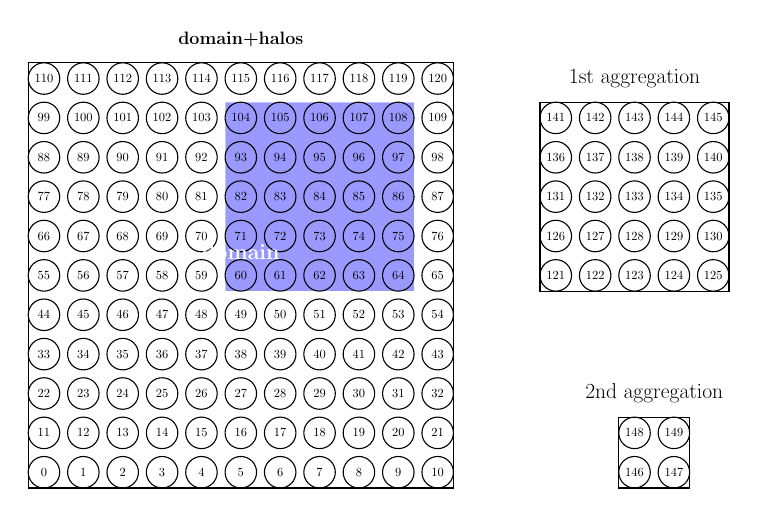
\begin{tikzpicture}[scale=\scale, every node/.style={scale=\scale*0.9}]
	\draw [white, fill=blue, opacity=0.4] (\halosize-\radius,\halosize-\radius) rectangle (\halosize+\domainsize-1+\radius, \halosize+\domainsize-1+\radius);
	\draw (0-\radius,0-\radius) rectangle (\totsize+\radius, \totsize+\radius);
	\draw (\ixo-\radius,\iyo-\radius) rectangle (\ixi+\radius, \iyi+\radius);
	\draw (\iixo-\radius,\iiyo-\radius) rectangle (\iixi+\radius, \iiyi+\radius);
		\foreach \y in {\thexo,...,\totsize} 
		{
			\foreach \x in {0,...,\totsize}
			{
				\draw (\x,\y) circle(\radius);
				\node at(\x,\y) {\thej};
				\addtocounter{j}{1};
			}	
		}
		\node [] at (\totsize*0.5,\totsize+1) {\Large\textbf {domain+halos}};
		\node [above, white] at (\totsize*0.5,\totsize*0.5+0.3) {\LARGE\textbf {domain}};
		\node [] at (0.5*\ixo+0.5*\ixi,\iyi+1) {\LARGE {1st aggregation}};
		\node [] at (0.5*\iixo+0.5*\iixi,\iiyi+1) {\LARGE {2nd aggregation}};
		\foreach \y in {\iyo,...,\iyi} 
		{
			\foreach \x in {\ixo,...,\ixi}
			{
				\draw (\x,\y) circle(\radius);
				\node at(\x,\y) {\thej};
				\addtocounter{j}{1};
			}	
		}
		\foreach \y in {\iiyo,...,\iiyi} 
		{
			\foreach \x in {\iixo,...,\iixi}
			{
				\draw (\x,\y) circle(\radius);
				\node at(\x,\y) {\thej};
				\addtocounter{j}{1};
			}	
		}
		
		
	
	\end{tikzpicture}
	
	\caption{Scheme for the indices of a process domain's data points in the underlying storage structure: the first section locates the domain itself with the surrounding halos. Directly hereafter follow aggregated values, always the complete coarsened domain at a time.}
\end{figure}


Here has to be:
- scheme how data is indexed
- scheme of aggergated data
- how fct Domain\_shape::index() works



\subsection{The class '\texttt{Shape}'}
Eventually the class \verb|Shape| combines the concepts presented in \ref{section_shape_halos}, \ref{section_shape_dom_dims} and \ref{section_shape_data_structure}. It indeed provides attributes to store the domain's \verb|begin| and \verb|end| - in the global coordinate system - and the extents \verb|domain_size|, \verb|total_size| and \verb|global_size|. Its function \verb|index| converts a point's three dimensional coordinates into the associated index in the data storage by 
\begin{codelisting1}
	return (x+halo_size_) + (y+halo_size_) * total_size[X] + 
				   (z+halo_size_) * total_size[X] * total_size[Y];
\end{codelisting1}
The remaining two function serves for accessing the \verb|halo_size|.
\begin{figure}[h!]
	\centering
	\def\scale{0.8}
	\def\x{0}
	\begin{tikzpicture}
	\umlclass[x=\x, y=0, scale=\scale]{Shape} {
		\# begin, end : \_vector\_t \\
		\# domain\_size, total\_size, global\_size : \_vector\_t \\
		\# halo\_size\_ : \_int\_t \\
		- class\_tag : std::string \\
	} {
		\umlvirt {+ index(\_coord\_t, \_coord\_t, \_coord\_t) constant : \_int\_t } \\
		{+ halo\_size() constant : constant \_int\_t\& } \\
		%+ size() constant : \_int\_t \\
	}
\end{tikzpicture}
%\caption{Attributes and relations among the storage classes \texttt{Storage}, \texttt{Storage\_const} and \texttt{Storage\_various}. }
\end{figure}


\subsection{Logical Position}
The logical position \verb|log_pos| of a process $P$ describes whether it has neighboring processes in a specified dimension. It is of interest for deciding whether a halo zone is among two processes or on the very outside as different behaviours may be desired. For its definition the declarations 
\begin{align}
	N^+_c &:= P\text{\footnotesize{ has a successive neighbour in dimension }} c \nonumber \\
	N^-_c &:= P\text{\footnotesize{ has a preceding neighbour in dimension }} c  \nonumber
\end{align}
are made. According to the combination of both the definition is made as
\begin{equation}
\text{\footnotesize\texttt{log\_pos[c]}} = 
\begin{cases} 
1 & if\quad N^+_c \land \lnot N^-_c  \\
0 & if\quad N^+_c \land  N^-_c  \\
-1 & if\quad \lnot N^+_c \land N^-_c  \\
-4 & if\quad \lnot N^+_c \land \lnot N^-_c  \\
\end{cases}
\end{equation}

\section{Policies}
\subsection{Data storage}
The abstract class \verb|Storage| works as a uniform interface to access the data. The base type is defined with template argument \verb|typename type__|. Its provides functions for constant and non-constant array access:
\begin{codelisting1}
	virtual type__& operator[](unsigned int) = 0;
	virtual const type__& operator[](unsigned int) const = 0;
\end{codelisting1}
Two concrete implementations are subclasses of the above-named. \verb|Storage_various| is the design to actually hold a value for every data point the domain. Therefore it keeps the memmber \verb|std::vector<type__> data| to store these values. The instanciation works via the constructor \verb|Storage_various(unsigned int size, type__ val=0)|, featuring a parameter for the size and an optional parameter to define a standard value. On the other \verb|Storage_const| facilitates the storage of a unique value as \verb|type__ data| and can be instanciated the analog way \verb|Storage_various(unsigned int, type__ val=0)|, though the size parameter does not have to be used. In distinguishing these two it is possible to save memory for cases where a data containing stores one constant value.
%\tikzumlset{font=\footnotesize}
\def\y{-5}
\def\x{5}
\def\dx{4}
\def\scale{0.6}
\begin{figure}[h!]
	\centering
	\begin{tikzpicture}
	\umlclass[x=\x, y=0, scale=\scale, template=type\_\_ : typename, type=abstract]{Storage} {} {
		\umlvirt { + operator[] (unsigned int) : type\_\_}\\
		\umlvirt { + operator[] (unsigned int) constant : constant type\_\_}\\
	}
	\umlclass[x=\x+\dx, y=\y, scale=\scale, template=type\_\_ : typename]{StorageVarious} {
		- data : std::vector\textless type\_\_ \textgreater \\
	}{
		+ Storage\_various(size : unsigned int, val : type\_\_ = 0) \\
		+ operator[] (index : unsigned int) : type\_\_\\
		+ operator[] (index : unsigned int) constant : constant type\_\_\\
	}
	\umlclass[x=\x-\dx, y=\y, scale=\scale, template=type\_\_ : typename]{StorageConst} {
		- data : type\_\_ \\
	}{
	+ Storage\_various(unsigned int, val : type\_\_ = 0) \\
	+ operator[] (unsigned int) : type\_\_\\
	+ operator[] (unsigned int) constant : constant type\_\_\\
	}
	\umlinherit{StorageConst}{Storage}
	\umlinherit{StorageVarious}{Storage}
\end{tikzpicture}
\caption{Attributes and relations among the storage classes \texttt{Storage}, \texttt{Storage\_const} and \texttt{Storage\_various}. }
\end{figure}

\subsection{Data access}
The abstract class \verb|Accessible| provides the data access interface. Its template parameters define the base type of the data \verb|typename type__| and the number of underlying storages \verb|unsigned int env__|. The general interface for constant and non-constant element access is then defined as 
\begin{codelisting1}
	virtual type__& get (_coord_t, _coord_t, _coord_t, _coord_t) = 0;
	virtual const type__& get (_coord_t, _coord_t, _coord_t, _coord_t) const = 0;
\end{codelisting1}
Its four parameters split in one to address a certain storage and three actual coordinates. For the case of one single underlying storage a partial template specialization \verb|Accessible<1, type__>| exists: The interface then specifies the same functions, yet only the three coordinate parameters are needed.

\section{\texttt{Processor\_grid}}
The class \verb|Processor_grid| reproduces the topology of the MPI processes. It provides functions to obtain the id of a process with relative coordinates to the calling process or the calling process' own:
\begin{codelisting1}
	int operator() ( int rel_x, int rel_y, int rel_z ) const;
	const int& operator() () const;
\end{codelisting1}
Furthermore it facilitates access to the process' absolute and the logical position in the grid, where the latter for a process $P$ is defined as 

\begin{codelisting1}
	const int& abs_pos(Coords c) const;
	const int& log_pos(Coords c) const;
	const std::array<int,3>& get_log_pos() const
\end{codelisting1}

\begin{codelisting1}
	const int& size ( Coords c ) const;
	const int& size () const;
	MPI_Comm& getCommunicator();
\end{codelisting1}


\section{\texttt{Type\_container}}

\subsection{Basic functionality}
The \verb|Type_container| can be instanciated by using its public constructor
\begin{codelisting1}
	Type_container(const Domain_shape& shape)
\end{codelisting1}	
and provides references to the send and receive types. The associated functions are called
\begin{codelisting1}
 	const MPI_Datatype& get_send_data_type(int x, int y, int z) const,
 	const MPI_Datatype& get_recv_data_type(int x, int y, int z) const.
\end{codelisting1}. 	
These types simplify the communication process as we do not any more need to copy the relevant data to or from buffers, respectively, in order to have it in a continuous piece of memory. This task is rolled out to other routines provided by MPI. It is only necessary to define and assemble the positions of all relevant memory locations. Moreover it is possible to interpret messages differently and therefore reconstruct the data to unequal positions on sending than on receiving side. The base MPI type of the values is handed via a template argument. Valid examples hereof are \verb|MPI_INT| or \verb|MPI_DOUBLE|; the total list can be found at \cite{MPI_docu}, tables 3.2 to 3.4. 

\subsection{MPI datatype construction routines}
\def\rI{0.07}
\def\rII{0.13}
\def\rect{0.3}
\begin{figure}	
	\centering
	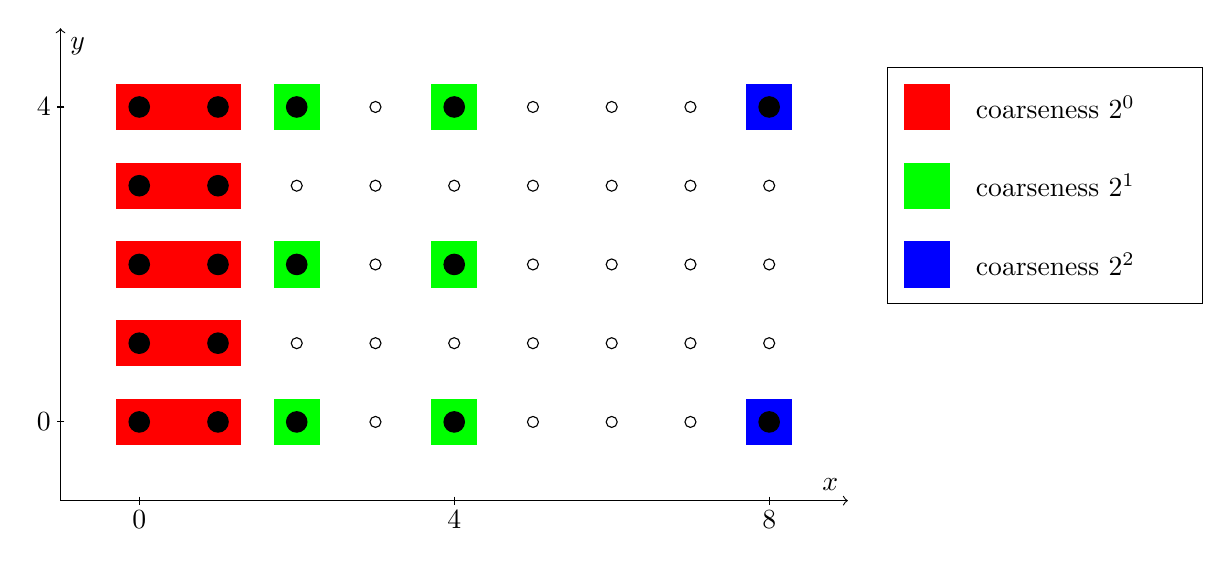
\begin{tikzpicture}
	\draw [->] (0,0) -> (10,0);
	\draw [->] (0,0) -> (0,6);
	\node [below right] at (0,6) {$y$};
	\node [above left] at (10,0) {$x$};
	\foreach \y in {1,..., 5} 
	\draw [white, fill=red] (1-\rect, \y-\rect) rectangle (2+\rect, \y+\rect);
	\foreach \x in { 1, ..., 9 }
	\foreach \y in { 1,..., 5 }
	\draw (\x,\y) circle (\rI);
	\foreach \x in { 1, 2 }
	\foreach \y in { 1,..., 5 }
	\draw [fill=black] (\x,\y) circle (\rII);
	\foreach \x in { 3, 5 }
	\foreach \y in {1, 3, 5}
	\draw [white, fill=green] (\x-\rect,\y-\rect) rectangle (\x+\rect,\y+\rect);
	\foreach \x in { 3, 5 }
	\foreach \y in {1, 3, 5}
	\draw [fill=black] (\x,\y) circle (\rII);
	\foreach \x in { 9 }
	\foreach \y in {1, 5}
	\draw [white, fill=blue] (\x-\rect,\y-\rect) rectangle (\x+\rect,\y+\rect);
	\foreach \x in { 9 }
	\foreach \y in {1, 5}
	\draw [fill=black] (\x,\y) circle (\rII);
	\draw (1,0.05) -> (1,-0.05);
	\node [below] at (1,0) {0};
	\draw (5,0.05) -> (5,-0.05);
	\node [below] at (5,0) {4};
	\draw (9,0.05) -> (9,-0.05);
	\node [below] at (9,0) {8};
	\draw (0.05,1) -> (-0.05,1);
	\node [left] at (0,1) {0};
	\draw (0.05,5) -> (-0.05,5);
	\node [left] at (0,5) {4};
	
	\draw (10.5,2.5) rectangle (14.5,5.5);
	\draw [white, fill=red] (11-\rect,5-\rect) rectangle (11+\rect,5+\rect);
	\node [right] at (11.5,5) {coarseness $2^0$};
	\draw [white, fill=green] (11-\rect,4-\rect) rectangle (11+\rect,4+\rect);
	\node [right] at (11.5,4) {coarseness $2^1$};
	\draw [white, fill=blue] (11-\rect,3-\rect) rectangle (11+\rect,3+\rect);
	\node [right] at (11.5,3) {coarseness $2^2$};
	\end{tikzpicture}
	\caption{Scheme for the block structure of the receive types: for the uncoarsened values ($2^0$) each line is one block; for all coarsened areas each value forms its own block.}
\end{figure}
MPI provides a variety of routines to construct customizes data types. In general one can define the parameters: 
\begin{itemize}
	\itemsep-0em
	\item \textit{count}: the number of blocks or elements the new type consists of
	\item \textit{length}: the number of consecutive elements in one block
	\item \textit{displacements} or \textit{stride}: the displacements of the blocks or elements or the constant stride among them
	\item \textit{oldtype}: the base type of a single element
\end{itemize}
The different constructors vary in whether these parameters are constant within the new type. \\
In the implementation at hand two new types are interleaved within one exchange type: the inner type bundles up all values of a certain coarseness; for example one inner type for all uncoarsened, one for all coarsened by $2^1$ and so on. Hence the parameters have the following characteristic: the blocklength remains constant (either the number of planes to be sent, or 1), we give an array of displacements with respect to the first point in the domain as in general there is no constant stride among the data points and the oldtype is the constant base type. For this case MPI provides the routine
\begin{codelisting1}
int MPI_Type_create_indexed_block(int count, int blocklength, const int displacements[], MPI_Datatype oldtype, MPI_Datatype *newtype).
\end{codelisting1}
In order to pack all types in one outer type we later use
\begin{codelisting1}
int MPI_Type_create_struct(int count, const int blocklengths[], const MPI_Aint displacements[], const MPI_Datatype types[], MPI_Datatype *newtype).
\end{codelisting1}
which is the simplest possibility to package the different inner types. In this routine allthough they all use the  point 0 for reference, it is necessary to specify a whole array of displacements as 0's. The same holds for the blocklength which is actually always 1 throughout the type.

\subsection{Receive types}
\begin{figure}
	\centering
	\def\scale{0.5}
	\begin{tikzpicture}[scale=\scale, every node/.style={scale=\scale*0.9}]
	\def\xsize{27}
	\def\ysize{27}
	\def\halosize{5}
	\def\fun{6}
	\def\r{0.4}
	\def\boxsize{0.45}
	\def\farbe{black}
	\draw[\farbe](1-\r,1-\r) rectangle (\xsize+\r, \ysize+\r);
	\draw[\farbe, dashed] (\xsize+\r, \ysize+\r) -- (\xsize+\r+1, \ysize+\r);
	\node[\farbe, right] at (\xsize+\r+1,\ysize+\r) {halo zones};
	\def\farbe{black}
	\draw[\farbe, fill=blue, opacity=0.1] (\halosize+1-\r, \halosize+1-\r) rectangle (\xsize-\halosize+\r,\ysize-\halosize+\r);
	\draw[\farbe, dashed] (\xsize-\halosize+\r,\ysize-\halosize+\r) -- (\xsize+\r+1, \ysize-\halosize+\r);
	\node[\farbe,right] at (\xsize+\r+1, \ysize-\halosize+\r) {domain};
	\newcounter{i}
	\def\test{\halosize+1}
	\foreach \y in {\halosize-1, \halosize}
	{
		\draw [white, fill=yellow] (\halosize+\boxsize, \y-\boxsize) rectangle (\xsize-\halosize+\boxsize, \y+\boxsize);
	}
	\foreach \y in {\halosize-2}
	{	
		\foreach \x in {6,8,...,22}
		{
			\draw [white, fill=green] (\x-0.45,\y-0.45) rectangle (\x+0.45,\y+\boxsize);
		}
	}
	\foreach \y in {1}
	{	\foreach \x in {6,10,...,24}
		{
			\draw [white, fill=red] (\x-\boxsize,\y-\boxsize) rectangle (\x+\boxsize,\y+\boxsize);
		}
	}
	\foreach \y in {\ysize-4,\ysize-3}
	{
		\draw [white, fill=yellow] (\halosize-2+\boxsize, \y-\boxsize) rectangle (\halosize+\boxsize, \y+\boxsize);
	}
	\draw [white, fill=green] (\halosize-3+\boxsize, \ysize-4-\boxsize) rectangle (\halosize-3+\boxsize+1, \ysize-4-\boxsize+1);
	\foreach \y in {1,...,\ysize} 
	{
		\foreach \x in {1,...,\xsize}
		{
			\draw (\x,\y) circle (\r);
			\node at (\x,\y) {\textbf{\arabic{i}}};
			\addtocounter{i}{1};	
		}
	}
	
	\end{tikzpicture}	
	\caption{;kj;}
\end{figure}



\subsection{Initialization process}
\begin{figure}
\centering
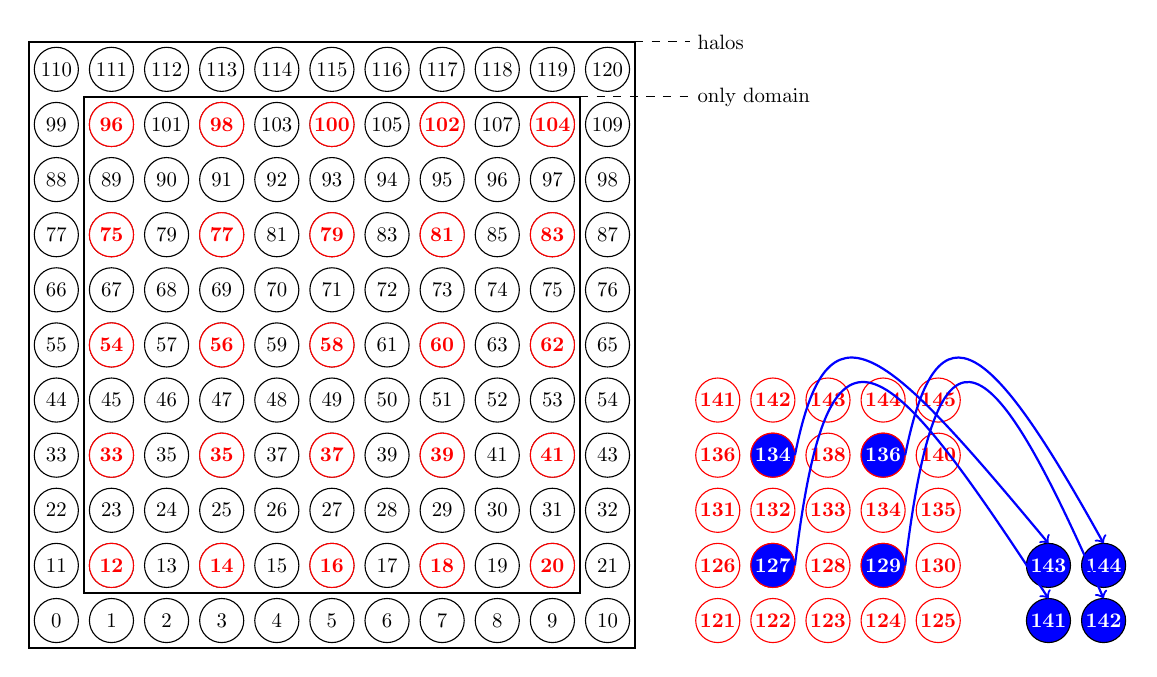
\begin{tikzpicture}[scale=0.7, every node/.style={scale=0.75}]
\draw [thick] (1.5,1.5) rectangle (10.5,10.5);
\draw [dashed] (10.5,10.5) -- (12.5,10.5);
\node [right] at (12.5,10.5) {only domain};
\draw [thick] (0.5,0.5) rectangle (11.5,11.5);
\draw [dashed] (11.5,11.5) -- (12.5,11.5);
\node [right] at (12.5,11.5) {halos};
%\newcounter{i}
\def\r{0.4}
	\foreach \y in {1,...,11} 
		\foreach \x in {1,...,11}
		{
			\draw (\x,\y) circle (\r);
			\node at (\x,\y) {\arabic{i}};
			\addtocounter{i}{1};			
		}
	\setcounter{i}{12}
	\foreach \y in {2,4,...,10} 
	{
		\foreach \x in {2,4,...,10}
		{
			\draw [red, fill=white] (\x,\y) circle (\r);
			\node [red, thick] at (\x,\y) {\textbf{\arabic{i}}};
			\addtocounter{i}{2};	
		}
		\addtocounter{i}{11};
	}
	\setcounter{i}{121}
	\foreach \y in {1,...,5} 
		\foreach \x in {13,...,17}
		{
			\draw [red, fill=white] (\x,\y) circle (\r);
			\node [red] at (\x,\y) {\textbf{\arabic{i}}};
			\stepcounter{i}		
		}
	\setcounter{i}{127}
	\foreach \y in {2,4}
	{
		\foreach \x in {14,16}
		{
			\draw [red, fill=blue] (\x,\y) circle (\r);
			\node [white, thick] at (\x,\y) {\textbf{\arabic{i}}};
			\addtocounter{i}{2};
		}	
		\addtocounter{i}{3};
	}
	\foreach \y in {1,2}
		\foreach \x in {19,20}
		{
			\draw [black, fill=blue] (\x,\y) circle (\r);
			\node [white, thick] at (\x,\y) {\textbf{\arabic{i}}};
			\stepcounter{i}	
		}
	\def\xo{14}
	\def\yo{2}
	\def\xi{19}
	\def\yi{1}
	\foreach \y in {0,2}
	{
		\foreach \x in {0,2}
		{
			\draw [->, thick, blue] (\xo+\x+\r,\yo+\y) .. controls (\xo+\x+1,7) and (\xo+\x+2,6) .. (\x/2+\xi,\y/2+\yi+\r);
		}
	}
\end{tikzpicture}	
\caption{;kj;}
\end{figure}
The constructor requires a reference to an object of \verb|Domain_shape|, which contains all necessary information about the size and halo properties of the process' domains. It is used to perform init routine \verb|void init_data_types(const Domain_shape&)|, which splits up in a phase for the send and the receive types, respecively. \\

\begin{figure}
	\centering
	\begin{tikzpicture}
	\umlclass[template=MPI\_Datatype]{Type\_container} {
		- send\_types : std::array\textless MPI\_Datatype, 27\textgreater  \\
		- recv\_types : std::array\textless MPI\_Datatype, 27\textgreater  \\
	}{
	\umlstatic{ - index(int, int, int) : int } \\
	- get\_send\_block\_number(const int\&, int, int, int, const Domain\_shape\&) : int \\
	- get\_recv\_block\_number(const int\&, int, int, int, const Domain\_shape\&) : int \\
	- get\_send\_block\_length(int, int, int, int, const Domain\_shape\&) : int \\
	- get\_recv\_block\_length(int, int, int, int, const Domain\_shape\&) : int \\
	- init\_data\_types(const Domain\_shape\&) : void \\
	- init\_recv\_types(int, std::array \textless MPI\_Datatype,27 \textgreater\& , const Domain\_shape\&) : void \\
	- init\_recv\_full\_types(std::array\textless MPI\_Datatype, 27 \textgreater\&, const Domain\_shape\&) : void \\
	- init\_send\_types(int, std::array\textless MPI\_Datatype, 27 \textgreater\& , const Domain\_shape \&) : void \\ \\
	+ Type\_container(const Domain\_shape\&)\\
	+ get\_send\_data\_type(int, int, int)const : const MPI\_Datatype\& \\
	+ get\_recv\_data\_type(int, int, int)const : const MPI\_Datatype\& \\
}
\end{tikzpicture}
\caption{Attributes of the class \texttt{Type\_container}. }
\end{figure}

\section{Logging}
For debugging purposes the logging facility offered by \cite{dobbs} is used.